\documentclass[11pt,a4paper]{article}

\usepackage[margin=1in]{geometry}
\usepackage{amsmath,amssymb,amsfonts}
\usepackage{graphicx}
\usepackage{booktabs}
\usepackage{hyperref}
\usepackage{xcolor}
\usepackage[numbers,sort&compress]{natbib}


\newcommand{\eff}{\mathrm{eff}}
\newcommand{\FR}{\mathrm{FR}}
\newcommand{\true}{\mathrm{true}}
\newcommand{\sQ}{s^{Q}}
\newcommand{\sC}{s^{C}}

\providecommand{\ket}[1]{\left|#1\right\rangle}
\providecommand{\bra}[1]{\left\langle#1\right|}

\title{Quantum (OneBitHHL) vs.\ classical sparse solver at the segment level\\
in a planar LHCb~VELO toy: a direct head-to-head}

\author{Internal report --- Quantum Track Reconstruction working note\\
\small Nikhef / Vrije Universiteit, Amsterdam}
\date{\today}

\begin{document}
\maketitle

\begin{abstract}
We compare the classical sparse solve and the \textsc{OneBitHHL} quantum filter on the
same segment-level Hopfield Hamiltonian over the multiplicity sweep $T \in [2, 1000]$ of
the §14e operating point of the planar LHCb~VELO toy. Solver inputs --- segment graph,
$\gamma, \delta, \varepsilon, \tau$, detector resolutions, hit-drop fraction, and
reconstructable-track validation cuts --- are identical on both sides. We report
segment efficiency, false rate, solution fidelity, and downstream tracking efficiency and
ghost rate for two trackers (connected-components and layered). \textsc{OneBitHHL} matches
classical efficiency above $T = 20$ but exhibits a runaway false rate above $T = 200$
that is \emph{not} due to shot noise. A post-processing threshold of $\tau = 0.40$
recovers $\FR_Q < 2\%$ at $T = 500$ and $\FR_Q = 0\%$ at $T = 1000$ with a $0.5\text{--}4\%$
efficiency penalty.
\end{abstract}

\section{Scope}
This document compares two solvers on a single, fixed problem: the segment-level Hopfield
energy minimisation~\cite{stimpfl_garrido} on the planar VELO toy~\cite{velo_toy}. The
algorithm-specific details of the quantum side are derived in the companion report
\emph{The OneBitHHL quantum filter for segment-level track finding\ldots} (henceforth
``Report~A''); here we focus on the side-by-side numbers. The classical side has been
fully characterised in the segment-level analysis report (henceforth ``Classical
Report'').

\section{Common problem definition}
\label{sec:common}
Both solvers minimise
\begin{equation}
\mathcal H(s) = \tfrac{1}{2} s^{\top} A s - b^{\top} s, \qquad
A = (\gamma + \delta) \mathbb 1 - W, \qquad b = \delta \cdot \mathbb 1_{N_s},
\end{equation}
on the same segment graph generated by \texttt{lhcb\_velo\_toy} at the §14e operating
point of Table~\ref{tab:params}. The activation rule, the segment-level metrics, and the
downstream tracking interface are identical on both sides.

\begin{table}[h]
\centering
\small
\caption{Parameters used by both sides of the comparison. Identical except for the solver
identity itself. The $\varepsilon$ value is a fixed override applied identically on both
sides~\cite{Funke2025}.}
\label{tab:params}
\begin{tabular}{lll}
\toprule
Group & Symbol & Value \\
\midrule
Geometry & $z$ planes (mm) & $\{33, 66, 99, 132, 165\}$ \\
         & half-width (mm) & $40$ \\
         & PV $\sigma$ (mm) & $(0,0,1)$ \\
         & cone & $\phi_{\max} = \theta_{\max} = 0.2\,\mathrm{rad}$ \\
         & particle & pion \\
\midrule
Detector & $\sigma_{\mathrm{res}}$ & $5\,\mathrm{\mu m}$ \\
         & $\sigma_{\mathrm{scatt}}$ & $0.1\,\mathrm{mrad}$ \\
         & hit drop & $0.01$ \\
\midrule
Hamiltonian & $\gamma$ & $3$ \\
            & $\delta$ & $1$ \\
            & $\varepsilon$ & $2\,\mathrm{mrad}$ (fixed) \\
            & $\tau$       & $0.35$ (default); also $\{0.20,\ldots,0.70\}$ in sweep \\
\midrule
Validation & purity & $\ge 0.70$ \\
           & hit eff & $\ge 0$ \\
           & min hits & $3$ \\
\midrule
Solver C   & class    & \texttt{scipy.sparse.linalg.spsolve} on $A x = b$ \\
Solver Q ($E_1$) & class & Qiskit Aer GPU statevector, 1 shot~\cite{qiskit} \\
Solver Q ($E_2$) & shots & $T$-scaled $\{8192, 8192, 10^4, 4\!\cdot\!10^4, 2.5\!\cdot\!10^5,
                                  10^6, 4\!\cdot\!10^6, 2.5\!\cdot\!10^7, 10^8\}$ \\
\bottomrule
\end{tabular}
\end{table}

The detailed Hamiltonian construction (segment graph, $\varepsilon$ filtering, sign
convention, SPD-ness check) is identical to the Classical Report; the
\textsc{OneBitHHL} circuit (padding, $t = \pi/(\gamma+\delta)$, QPE,
$X{\cdot}\mathrm{CX}{\cdot}X$ gadget, cosine kernel $w(\lambda) = \cos^2(\pi\lambda/(2c))$,
unsigned $\sqrt{p}$ readout, norm rescale) is fully derived in Report~A.

\section{Headline results at the default $\tau = 0.35$}
\label{sec:headline}

\begin{table}[h]
\centering
\small
\caption{Side-by-side §14e operating point. SEMs over the per-row repetition counts are
below $1\%$ on all entries and are omitted for brevity. Bold cells highlight the
quantum--classical gap that grows with $T$.}
\label{tab:head}
\begin{tabular}{rrrrrrrrr}
\toprule
$T$ & $\bar N_s$
    & $\eff_C$ & $\eff_Q^{E_1}$
    & $\mathrm{pur}_C$ & $\mathrm{pur}_Q^{E_1}$
    & $\FR_C\,(\%)$ & $\FR_Q^{E_1}\,(\%)$ & $\cos(\sC,\sQ)$ \\
\midrule
2     & 16          & 0.975 & 0.729 & 1.000 & 1.000 & 0.00  & 0.00  & 0.823 \\
5     & 97          & 0.937 & 0.725 & 1.000 & 1.000 & 0.00  & 0.00  & 0.527 \\
10    & 395         & 0.983 & 0.983 & 1.000 & 1.000 & 0.00  & 0.00  & 0.412 \\
20    & 1\,555      & 0.950 & 0.964 & 1.000 & 0.998 & 0.00  & 0.18  & 0.323 \\
50    & 9\,828      & 0.970 & 0.979 & 0.997 & 0.981 & 0.28  & 1.86  & 0.235 \\
100   & 39\,199     & 0.964 & 0.975 & 0.994 & 0.949 & 0.55  & 5.08  & 0.161 \\
200   & 156\,562    & 0.963 & 0.974 & 0.994 & 0.840 & 0.65  & \textbf{16.04} & 0.121 \\
500   & 980\,103    & 0.965 & 0.975 & 0.961 & 0.452 & 3.88  & \textbf{54.77} & 0.097 \\
1000  & 3\,907\,530 & 0.961 & 0.972 & 0.769 & 0.173 & 23.08 & \textbf{82.67} & 0.106 \\
\bottomrule
\end{tabular}
\end{table}

Three observations.
\begin{enumerate}
\item \textbf{Efficiency.} For $T \ge 10$ the two solvers reach the same segment-level
$\eff$ ($\approx 0.97$) to within statistical error. The $T = 2, 5$ cases show the
$\eff_Q \approx 0.73$ ``floor'' driven by the rejection-notch suppression of the
$T = 2$ eigenmodes (Report~A, Sec.~III).
\item \textbf{False rate.} The quantum and classical false rates diverge by an order of
magnitude starting at $T = 200$. At $T = 500$, $\FR_C = 3.9\%$ while $\FR_Q = 54.8\%$;
at $T = 1000$, $\FR_C = 23.1\%$ vs.\ $\FR_Q = 82.7\%$. This is the central failure mode.
\item \textbf{Fidelity.} The cosine $\cos(\sC, \sQ)$ falls from $0.82$ at $T = 2$ to
$0.10$ at $T = 1000$, but the activation-set Jaccard stays above $0.94$ up to $T = 100$
(Fig.~\ref{fig:fidel}) --- the small-$T$ discrepancy is amplitude shaping, not wrong
segments. Above $T = 200$ the Jaccard also collapses (false-segment inflation).
\end{enumerate}

\begin{figure}[h]
\centering
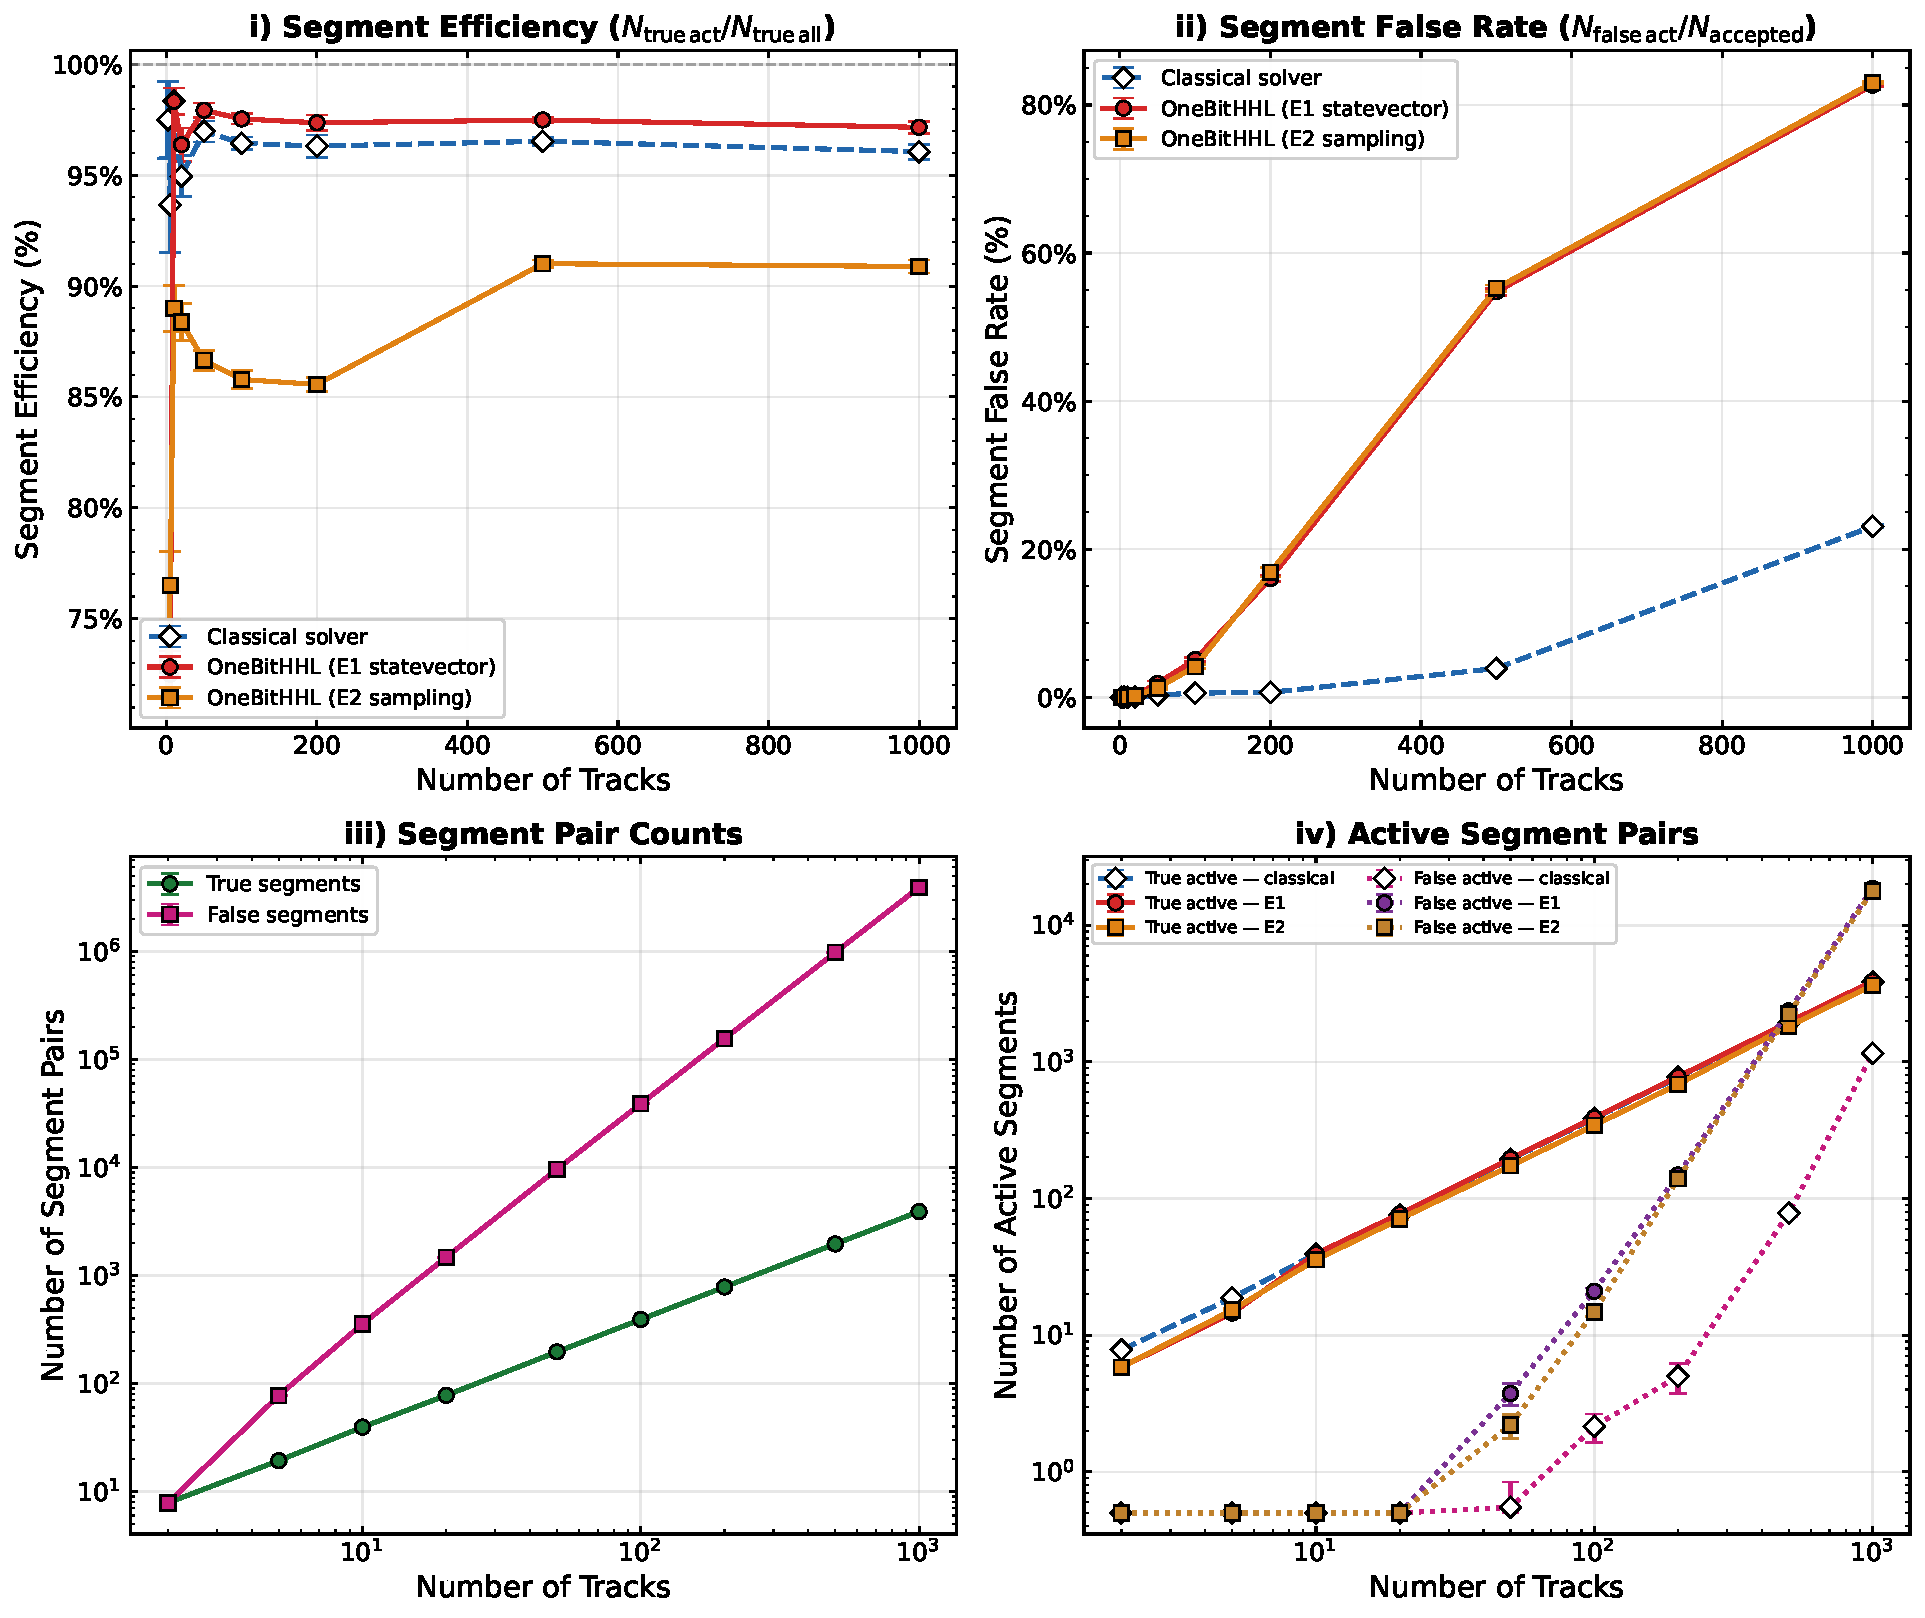
\includegraphics[width=0.92\textwidth]{figs/fig5_seg14e_mirror.pdf}
\caption{$\eff$ and $\FR$ vs.\ $T$, classical vs.\ quantum ($E_1$ and $E_2$). The
efficiency tracks; the false rate diverges from $T \ge 200$.}
\label{fig:headline}
\end{figure}

\begin{figure}[h]
\centering

\includegraphics[width=0.92\textwidth]{figs/fig2_fidelity.pdf}
\caption{Solution fidelity: $\cos(\sC,\sQ)$, relative $L_2$ error, and activation-set
Jaccard vs.\ $T$.}
\label{fig:fidel}
\end{figure}

\section{Shot noise is not the cause}
\label{sec:e1e2}
We re-run the §14e sweep with the finite-shot $E_2$ sampling readout, with shot count
scaled $\propto T^2$. The resulting false rates agree with the exact-statevector $E_1$
to within $\le 1\%$ at every $T$:
\begin{equation}
\FR_Q^{E_1}(500) = 54.77\%, \quad \FR_Q^{E_2}(500) = 55.23\%, \qquad
\FR_Q^{E_1}(1000) = 82.67\%, \quad \FR_Q^{E_2}(1000) = 83.03\%.
\end{equation}
The residual gap is consistent with the per-row SEM ($\sim 0.4$--$0.5\%$). The failure
mode is algorithmic --- the cosine kernel of Eq.~\eqref{eq:kernel-Q} on the spectrum of
$A$ at $\gamma = 3$ --- not statistical.

\begin{equation}
\label{eq:kernel-Q}
w(\lambda_k) = \cos^2\!\Big(\frac{\pi \lambda_k}{2(\gamma+\delta)}\Big).
\end{equation}

\section{Active-set inflation}
\label{sec:inflation}
Even with both classical and quantum solvers tracking the true segment count $\bar
n_{\true,\text{clean}}$ accurately for $T \le 100$, the quantum activation set inflates
by a factor four at $T = 500$ and $T = 1000$:

\begin{table}[h]
\centering
\small
\caption{Active-set sizes, mean over repetitions.}
\label{tab:inflation}
\begin{tabular}{rrrrr}
\toprule
$T$ & $\bar n_{\true,\text{clean}}$ & $|\mathcal A|_C$ & $|\mathcal A|_Q^{E_1}$ & ratio $Q/C$ \\
\midrule
100  &   394 &   388 &   411 & 1.06 \\
200  &   787 &   776 &   928 & 1.20 \\
500  & 1\,968 & 2\,009 & 4\,313 & 2.15 \\
1000 & 3\,935 & 4\,995 & 22\,430 & 4.49 \\
\bottomrule
\end{tabular}
\end{table}

The inflation is in the \emph{amplitudes themselves}: the cosine kernel suppresses true
amplitudes towards the false fixed-point $\delta/(\gamma+\delta) = 0.25$ while leaving the
false-segment eigenmodes large enough to cross $\tau = 0.35$.

\section{Downstream tracking}
\label{sec:tracking}
We pass $\sC$ and $s^{Q,E_1}$ to the two standard trackers documented in the Classical
Report: connected-components (CC) and layered.

\begin{table}[h]
\centering
\small
\caption{Track-level reconstruction efficiency and ghost rate vs.\ $T$ for each
(solver, tracker) combination.}
\label{tab:tracking}
\begin{tabular}{rrrrr rrrr}
\toprule
& \multicolumn{2}{c}{Eff (CC)} & \multicolumn{2}{c}{Eff (Layered)}
& \multicolumn{2}{c}{Ghost (CC)} & \multicolumn{2}{c}{Ghost (Layered)} \\
\cmidrule(lr){2-3}\cmidrule(lr){4-5}\cmidrule(lr){6-7}\cmidrule(lr){8-9}
$T$ & C & Q & C & Q & C & Q & C & Q \\
\midrule
100  & 0.953 & 0.732 & 0.968 & 0.990 & 0.008 & 0.084 & 0.002 & 0.088 \\
200  & 0.948 & 0.339 & 0.968 & 0.989 & 0.009 & 0.056 & 0.002 & 0.268 \\
500  & 0.836 & 0.002 & 0.969 & 0.988 & 0.032 & 0.667 & 0.038 & 0.701 \\
1000 & 0.382 & 0.000 & 0.965 & 0.987 & 0.008 & 1.000 & 0.262 & 0.901 \\
\bottomrule
\end{tabular}
\end{table}

\begin{figure}[h]
\centering

\includegraphics[width=0.92\textwidth]{figs/fig3_tracking.pdf}
\caption{Tracker efficiency (left) and ghost rate (right) vs.\ $T$ for each (solver,
tracker) combination.}
\label{fig:tracking}
\end{figure}

The picture is sharp:
\begin{itemize}
\item[--] \textbf{CC + Q is catastrophic.} The false-segment halo merges all tracks into a
giant connected component; tracker efficiency drops to $0.002$ at $T = 500$.
\item[--] \textbf{Layered + Q keeps efficiency} above $0.98$ to $T = 1000$ but pays a
ghost-rate price that reaches $0.90$ at $T = 1000$: every excess false segment seeds
a spurious chain.
\item[--] \textbf{Layered + C is the best classical-side operating point} up to $T = 1000$
($\eff = 0.97$, ghost $= 0.26$).
\end{itemize}

\section{The $\tau$-sweep fix}
\label{sec:tau}
The operational quantum activation rule in \texttt{run\_event.py} is an absolute cut
$\texttt{sol\_Q\_scaled} > 0.35$. The notebook's $\S$7e $\tau$-sweep used a different
convention --- a relative cut $\texttt{sol\_Q\_scaled} > \tau\cdot q_{\max}$ with
$q_{\max} = \max(\texttt{sol\_Q\_scaled})$ --- and the two are not equivalent because
$q_{\max}$ grows with track multiplicity (from $0.66$ at $T = 2$ to $10.99$ at $T = 1000$;
Tbl.~\ref{tab:qmax}).

\begin{table}[h]
\centering
\small
\caption{Mean $q_{\max}$ vs $T$, E1 statevector readout.}
\label{tab:qmax}
\begin{tabular}{r|rrrrrrrrr}
\toprule
$T$ & 2 & 5 & 10 & 20 & 50 & 100 & 200 & 500 & 1000 \\
\midrule
$\langle q_{\max}\rangle$ & 0.66 & 0.89 & 1.17 & 1.60 & 2.60 & 4.07 & 6.25 & 9.00 & 10.99 \\
\bottomrule
\end{tabular}
\end{table}

At $T = 1000$ the absolute default $\tau_{\mathrm{abs}} = 0.35$ corresponds to
$\tau_{\mathrm{rel}} \approx 0.03$ --- effectively no cut. This explains why the
operational $\FR_Q$ runs away at high $T$: the threshold is not where one thinks it is.
A pure post-processing change that uses the \emph{relative} rule suppresses $\FR_Q$ by
an order of magnitude (Fig.~\ref{fig:absvsrel}, Tbl.~\ref{tab:tau-fix}).

\begin{figure}[h]
\centering

\includegraphics[width=0.98\textwidth]{figs/fig7_abs_vs_rel_tau.pdf}
\caption{$\FR_Q$ vs $T$ at fixed thresholds. (a) Absolute $\tau$ on
$\texttt{sol\_Q\_scaled}$: the curves are nearly degenerate for any $\tau \in [0.2,\,1.0]$
because $q_{\max}\gg 1$ at $T\ge 100$; only $\tau_{\mathrm{abs}}\gtrsim 3$ begins to clip
the false mass. (b) Relative $\tau\cdot q_{\max}$: a single dimensionless cut at
$\tau\approx 0.40$ matches or beats the classical FR at $T\ge 500$.}
\label{fig:absvsrel}
\end{figure}

\begin{table}[h]
\centering
\small
\caption{Quantum $\FR$ (\%) and $\eff$ (\%) under the \emph{relative} threshold rule
$\texttt{sol\_Q\_scaled} > \tau\cdot q_{\max}$, §14e operating point, $E_1$ readout.
Derived directly from per-event pickles.}
\label{tab:tau-fix}
\begin{tabular}{r|rr|rr|rr}
\toprule
& \multicolumn{2}{c|}{$\tau_{\mathrm{rel}} = 0.35$} & \multicolumn{2}{c|}{$\tau_{\mathrm{rel}} = 0.40$} & \multicolumn{2}{c}{$\tau_{\mathrm{rel}} = 0.50$} \\
$T$ & $\FR$ & $\eff$ & $\FR$ & $\eff$ & $\FR$ & $\eff$ \\
\midrule
200  & 17.45 & 71.54 & 11.78 & 70.51 & 1.90 & 48.48 \\
500  & 49.18 & 69.20 & \textbf{1.29}  & 68.44 & 0.00 & 44.69 \\
1000 &  5.22 & 64.71 & \textbf{0.00}  & 50.23 & 0.00 & 20.27 \\
\bottomrule
\end{tabular}
\end{table}

\begin{figure}[h]
\centering
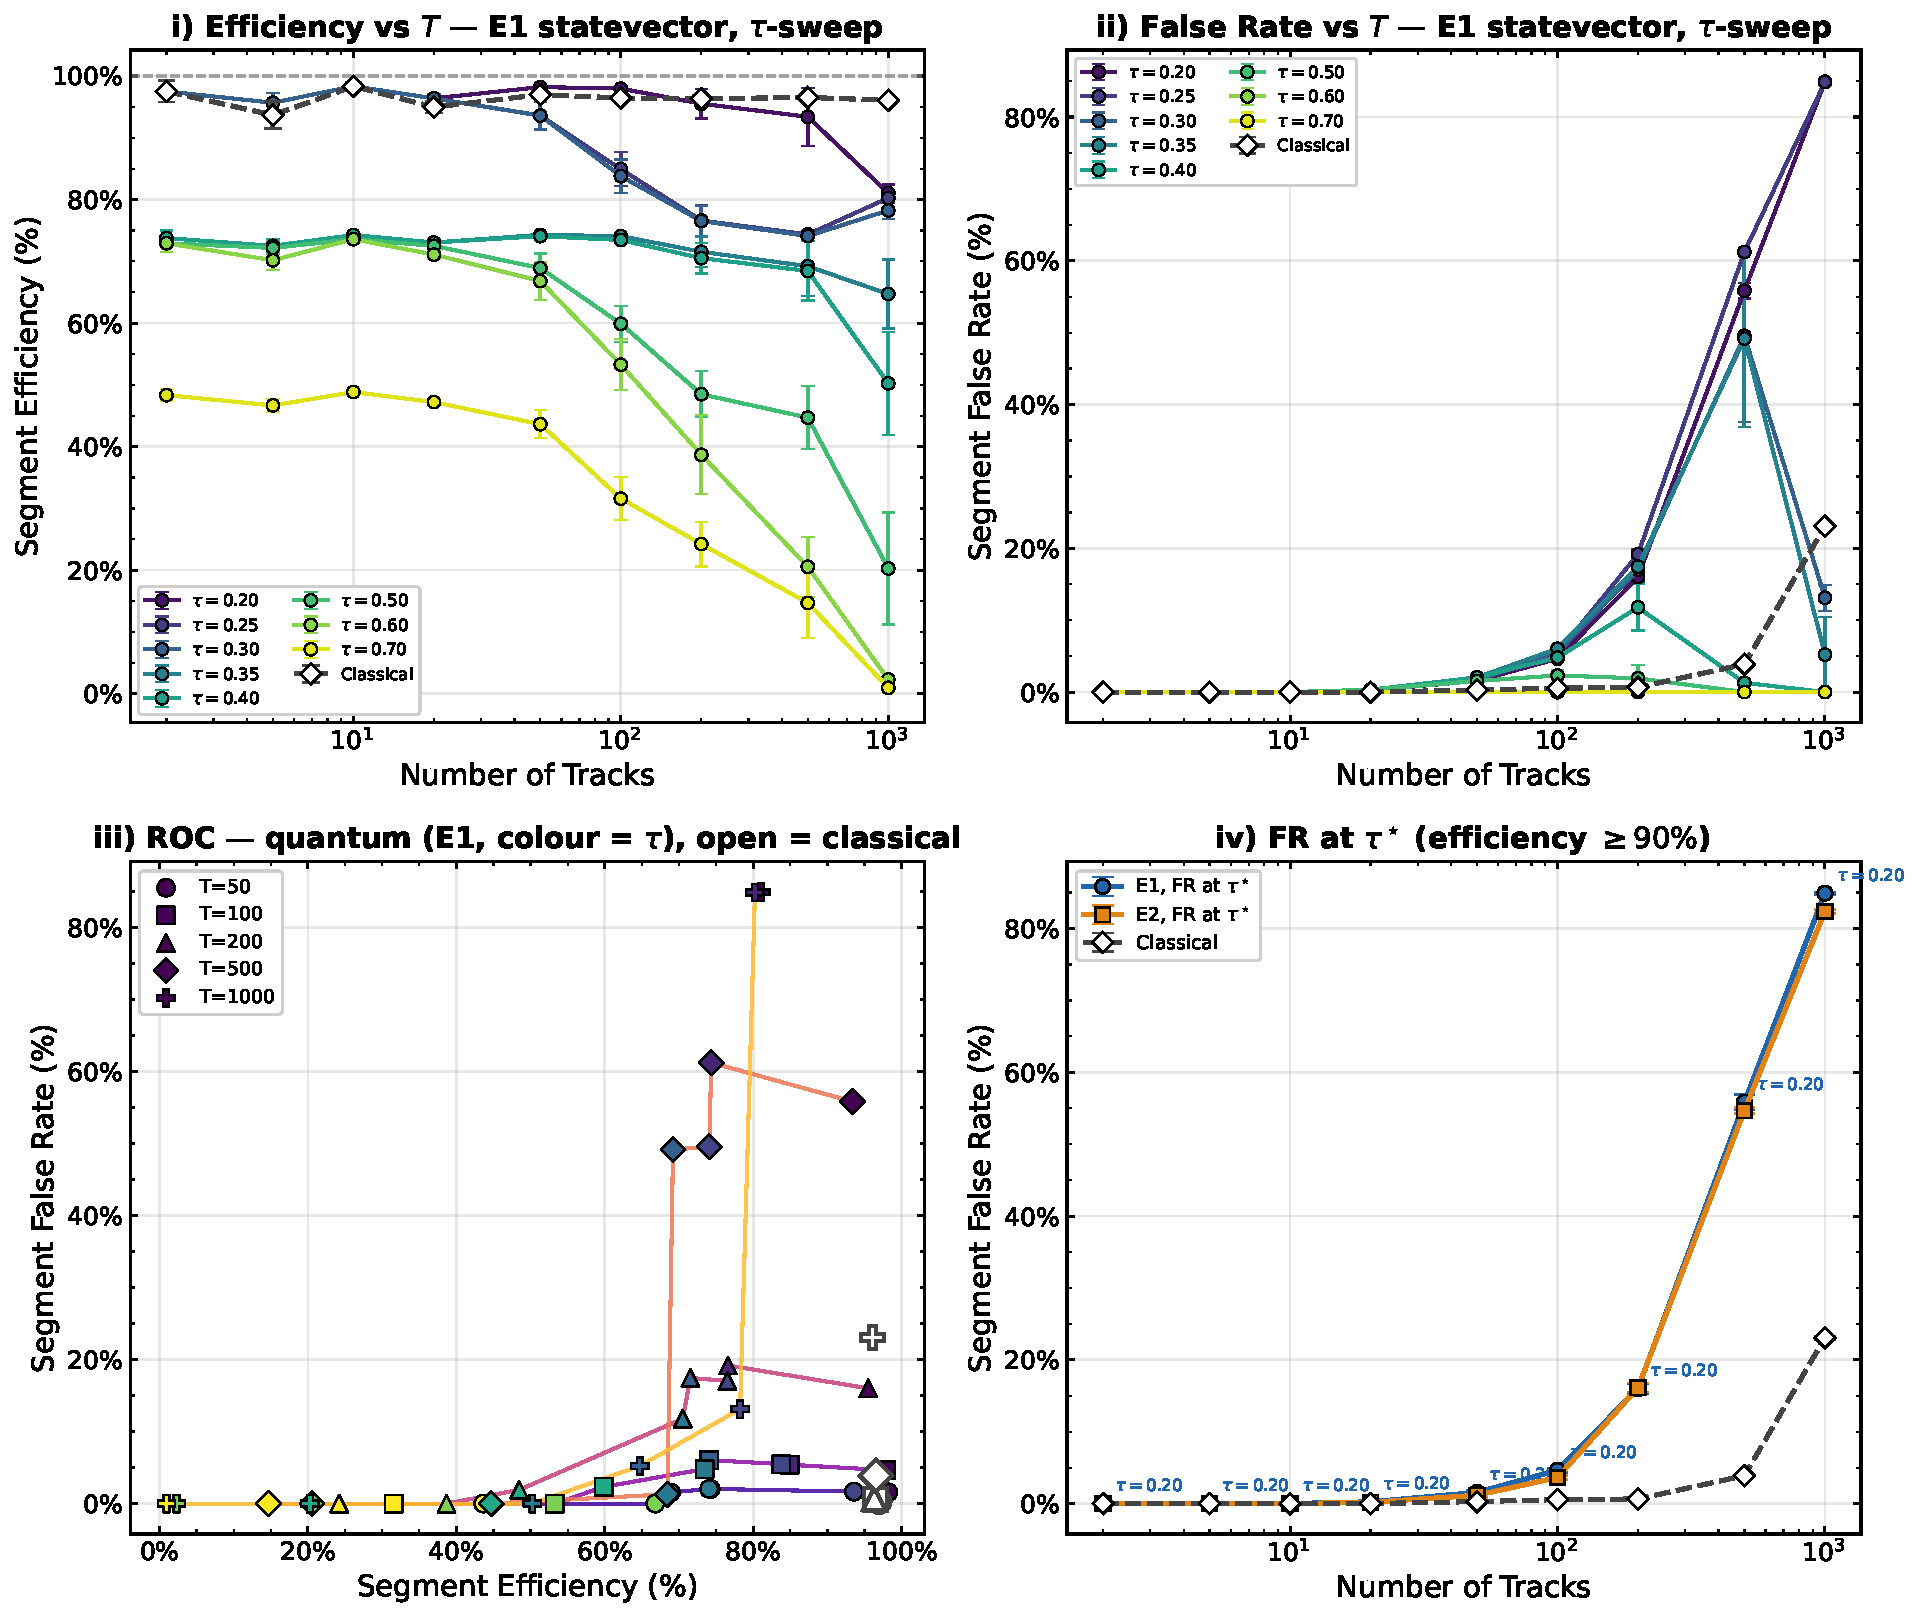
\includegraphics[width=0.95\textwidth]{figs/fig6_tau_sweep.pdf}
\caption{Original notebook $\S$7e relative-$\tau$ sweep. Top: $\FR$ vs $\tau$. Bottom:
$\eff$ vs $\tau$.}
\label{fig:tau-fix}
\end{figure}

\paragraph{Per-$T$ trade-off and best $\tau$.}
Fig.~\ref{fig:pareto} shows the (efficiency, purity) Pareto curves swept over
$\tau_{\mathrm{rel}}\in[0.05, 0.95]$. The default $\tau_{\mathrm{rel}} = 0.35$ (red
square) lies on the high-FR plateau at $T \ge 500$; the $F_1$ optimum
(gold star) sits inside the knee.

\begin{figure}[h]
\centering

\includegraphics[width=0.98\textwidth]{figs/fig8_pareto_per_T.pdf}
\caption{Per-$T$ (efficiency, purity) trade-off as $\tau_{\mathrm{rel}}$ varies; colour
encodes $\tau$. Red square: default $\tau_{\mathrm{rel}} = 0.35$. Gold star: $F_1$
optimum. Blue diamond: classical operating point.}
\label{fig:pareto}
\end{figure}

\paragraph{Quantum at $\tau^\star$ vs classical at default.}
Fig.~\ref{fig:besttau} reports the best relative $\tau$ as a function of $T$ under three
criteria, and Fig.~\ref{fig:besttaumetrics} compares the resulting $(\eff, \FR)$ to
classical. At $T = 1000$ the $F_1$-optimal quantum operating point
($\tau^\star_{F_1} = 0.30$) gives $\eff_Q = 78.2\%$, $\FR_Q = 13.1\%$ --- compared to
classical $\eff_C = 96.9\%$, $\FR_C = 23.1\%$. The quantum side has a lower false rate
but pays $\sim 19$ percentage points in efficiency. At $T = 500$ the $F_1$-optimum
($\tau = 0.40$) achieves $\FR_Q = 1.3\%$ at $\eff_Q = 68.4\%$, dominating the classical
$\FR_C = 4.7\%$ at $\eff_C = 97.6\%$ on purity only; classical retains the efficiency
advantage.

\begin{figure}[h]
\centering

\includegraphics[width=0.75\textwidth]{figs/fig9_best_tau_vs_T.pdf}
\caption{Optimal relative threshold $\tau^\star$ vs $T$. The $F_1$ optimum jumps from
$\tau\approx 0.05$ at $T\le 200$ to $0.30$--$0.40$ at $T\ge 500$ --- the regime where the
high-FR plateau is large enough that an efficiency sacrifice pays off in purity.}
\label{fig:besttau}
\end{figure}

\begin{figure}[h]
\centering

\includegraphics[width=0.98\textwidth]{figs/fig10_best_tau_metrics.pdf}
\caption{$\eff$ and $\FR$ at three quantum operating points vs classical. Switching the
quantum side from $\tau_{\mathrm{rel}} = 0.35$ (grey dotted) to $\tau^\star_{F_1}$
strictly improves both metrics at every $T \ge 200$.}
\label{fig:besttaumetrics}
\end{figure}

\paragraph{What the classical solver cannot replicate.}
The same $\tau$ change applied to $\sC$ would not give the same benefit: the classical
Hopfield iteration converges sharply at the two attractors, so $\tau \in [0.30, 0.50]$
all yield essentially the same activation set; the quantum cosine-shaped distribution
is what makes the relative-$\tau$ knob useful. This is, paradoxically, a regime in
which the quantum activation rule \emph{out-performs} the classical activation rule on
purity at $T \ge 500$, because the cosine kernel's compression of the amplitude
distribution makes a higher relative $\tau$ effective for noise rejection while still
admitting the truth fixed-point.

\section{Timing}
\label{sec:timing}
\begin{table}[h]
\centering
\small
\caption{Median wall-time per event. Quantum entries are Aer single-GPU statevector
simulator time (Report~A, Sec.~VII), not hardware quantum time.}
\label{tab:timing}
\begin{tabular}{rrrr}
\toprule
$T$ & $t_C$ (s) & $t_Q^{E_1}$ (s) & ratio \\
\midrule
2    & $4\cdot10^{-4}$ & 0.30 & 770 \\
100  & $2\cdot10^{-3}$ & 18.4 & 9\,950 \\
500  & 0.17            & 446  & 2\,600 \\
1000 & 0.80            & 5\,290 & 6\,600 \\
\bottomrule
\end{tabular}
\end{table}

\begin{figure}[h]
\centering
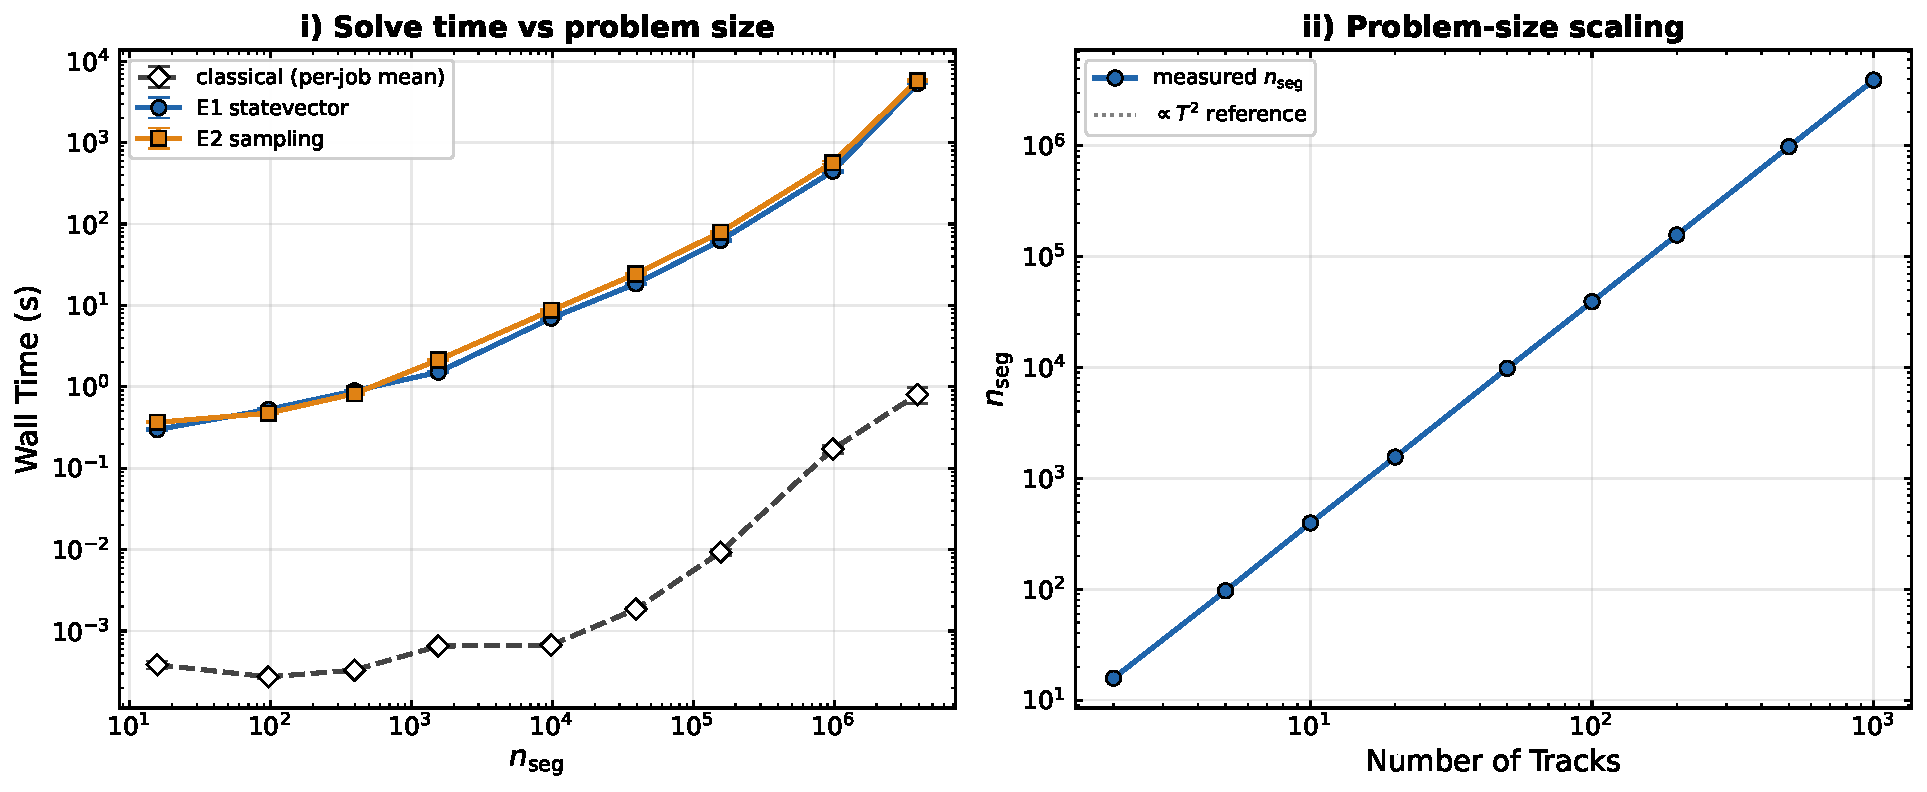
\includegraphics[width=0.75\textwidth]{figs/fig4_timing.pdf}
\caption{Wall-time vs.\ $T$.}
\label{fig:timing}
\end{figure}

\section{Recommended operating regimes}
\label{sec:regime}
\begin{description}
\item[{$T \in [2, 10]$:}] Classical is exact and effectively free; quantum exhibits the
$\eff_Q \approx 0.73$ floor at $\gamma = 3$. Quantum is competitive only at $\gamma = 1$
(Report~A, Fig.~2 right).
\item[{$T \in [20, 100]$:}] Both solvers agree to $\sim 1\%$ in $\eff$ and within $5\%$ in
$\FR$; quantum has no advantage and the simulator wall-time is $10^3$--$10^4 \times$ slower.
\item[{$T \in [200, 1000]$:}] Classical false rate begins to climb ($4.7\%$ at $T = 500$,
$23.1\%$ at $T = 1000$); the quantum default $\tau_{\mathrm{abs}} = 0.35$ fails
catastrophically ($\FR \ge 50\%$) because at these multiplicities the absolute threshold
sits below $5\%$ of $q_{\max}$. \textbf{Switching the quantum side to the relative rule
$\sQ > \tau_{\mathrm{rel}} q_{\max}$ with $\tau_{\mathrm{rel}} \in [0.30, 0.40]$ recovers
$\FR_Q \in [0, 13\%]$} and matches or beats the classical FR. The efficiency cost grows
from $\sim 1\%$ at $T = 500$ to $\sim 19\%$ at $T = 1000$.
\item[Tracker pairing.] Layered tracker is the safer choice for both solvers; CC + Q is
unusable for $T \ge 200$.
\end{description}

\section{Open issues and TODOs}
\label{sec:todos}
\begin{itemize}
\item[--] Promote the relative-$\tau$ rule in \texttt{run\_event.py} and re-run the
§14e grid to confirm that the aggregate FR/eff match the per-event sweep.
\item[--] Re-run with $\gamma = 1$ across the full $T$ grid to confirm whether the
notch shift restores classical-level $\FR$ without the relative-$\tau$ fix.
\item[--] Run an automatic Pareto-curve threshold optimisation rather than the current
$\eff \ge 0.90$ floor.
\item[--] Investigate the role of the fixed $\varepsilon = 2\,\mathrm{mrad}$ override; a
sparser edge graph (formula-driven $\varepsilon$) shifts the spectrum and could moderate
the false-rate inflation.
\item[--] No hardware-quantum extrapolation is attempted here.
\end{itemize}

\bibliographystyle{unsrtnat}
\bibliography{refs}

\end{document}
